
\documentclass[a4paper,12pt]{article}
\usepackage[a4paper,top=1.3cm,bottom=2cm,left=1cm,right=1cm,marginparwidth=0.75cm]{geometry}

\usepackage{mathtext} 
\usepackage{setspace}
\usepackage{tabularx}
\usepackage{cmap}
\usepackage{longtable}
\usepackage{icomma}
\usepackage{euscript}
\usepackage{float}
\usepackage{cutwin}
\usepackage{mathrsfs}
\usepackage{adjustbox}
\usepackage{dashbox}
\usepackage[normalem]{ulem}
\usepackage[T1,T2A]{fontenc}	
\usepackage[utf8]{inputenc}         
\usepackage[english,russian]{babel} 
\usepackage[babel=true]{microtype}
\RequirePackage[T1]{fontenc}
\usepackage{amsmath,amsfonts,amssymb,amsthm,mathrsfs,mathtools} 
\usepackage{xcolor}         
\usepackage{enumitem}     
\usepackage{xpatch}       
\usepackage{cancel}                  
\usepackage{upgreek}                 
\usepackage{lipsum}                  
\usepackage[version=4]{mhchem}       
\usepackage{multirow}                
\usepackage{stackengine}             
\usepackage{tikz}         
\usepackage{hyperref}
\hypersetup{colorlinks=true,urlcolor=blue}       
\usetikzlibrary{positioning}         
\usepackage{titletoc}                
\usepackage{titlesec}                
\usepackage{wrapfig}                 
\usepackage{chngcntr}              
\usepackage{fancyhdr}                
\usepackage{makecell}                
\usepackage{indentfirst}             
\usepackage{tocloft}                 
\usepackage{soul}                   
\usepackage[stable]{footmisc}       
\usepackage{subfig}                  

\mathtoolsset{showonlyrefs=true}


\theoremstyle{definition}
\newtheorem*{definition}{Определение}
\newtheorem{statement}{Предложение}[section]
\newtheorem{lemma}{Лемма}[section]
\newtheorem{theorem}{Теорема}[section]
\newtheorem*{theoremn}{Теорема}
\newtheorem*{corollary}{Следствие}
\newtheorem*{example}{Пример}
\newtheorem*{note}{Замечание}
\newtheorem*{problem}{Задача}


\counterwithout{footnote}{section}\DeclareRobustCommand{\divby}{%
	\mathrel{\text{\vbox{\baselineskip.65ex\lineskiplimit0pt\hbox{.}\hbox{.}\hbox{.}}}}%
}

\newcommand{\dotpr}[2]{\bra{#1}\ket{#2}}
\let\AA\relax
\let\emptyset\varnothing
\DeclareMathOperator*{\esssup}{ess sup}
\DeclareMathOperator*{\ord}{ord}
\DeclareMathOperator*{\supp}{supp}
\DeclareMathOperator*{\pr}{pr}
\DeclareMathOperator*{\Ker}{Ker}
\DeclareMathOperator*{\Vol}{Vol}
\DeclareMathOperator*{\rg}{rk}
\DeclareMathOperator*{\Ima}{Im}
\DeclareMathOperator*{\Alt}{Alt}
\DeclareMathOperator*{\Sym}{Sym}
\newcommand{\eqdef}{\stackrel{\text{\tiny{def}}}{=}}
\newcommand{\pp}{\partial}
\newcommand{\AA}{\mathcal{A}}
\newcommand{\BB}{\mathcal{B}}
\newcommand{\MM}{\mathbb{M}}
\newcommand{\NN}{\mathbb{N}}
\newcommand{\ZZ}{\mathbb{Z}}
\newcommand{\QQ}{\mathbb{Q}}
\newcommand{\RR}{\mathbb{R}}
\newcommand{\CC}{\mathbb{C}}
\newcommand{\FFF}{\mathbb{F}}
\newcommand{\DD}{\mathcal{D}}
\newcommand{\FF}{\mathcal{F}}
\newcommand{\sS}{\mathcal{S}}
\newcommand*\circled[1]{\tikz[baseline=(char.base)]{
		\node[shape=circle,draw,inner sep=2pt] (char) {#1};}}

\graphicspath{ {./images/2.5.1} }


\title{Измерение коэффициента поверхностного натяжения жидкости (2.5.1)}
\author{Павлушкин Вячеслав}
\date{\today}


\begin{document}
	\maketitle
	\section{Аннотация}
	В данной работе мы находим коэффициент поверхностного натяжения, с помощью иглы, колб с жидкостями и аспиратора, создающего разность давления.
	\section{Введение}
	\noindent\textbf{Цель работы:}
	1) измерение температурной зависимости  коэффициента поверхностного натяжения дистиллированной воды с использованием известного коэффициента поверхностного натяжения спирта; 2) определение полной поверхностной энергии  и теплоты, необходимой для изотермического образования единицы  поверхности жидкости  при различной температуре.
	
	\bigskip
	\noindent\textbf{В работе используются:} прибор  Ребиндера  с термостатом и микроманометром; исследуемые жидкости; стаканы; микроскоп.
	\section{Теоретические сведения}
	
	Наличие поверхностного слоя приводит к различию давлений по разные стороны от искривленной границы раздела двух сред.  Для сферического пузырька с воздухом  внутри жидкости избыточное давление дается формулой Лапласа:
	
	\begin{equation}
		\Delta P = P_{int} - P_{ext} = \frac{2\sigma}{r},
		\label{key}
	\end{equation}
	где $ \sigma $ -- коэффициент поверхностного натяжения, $ P_{int} $ и $ P_{ext} $ -- давление внутри пузырька и снаружи, $ r $ -- радиус кривизны поверхности раздела двух фаз. Эта формула лежит в основе предлагаемого метода определения коэффициента поверхностного натяжения жидкости. Измеряется давление $ \Delta P $, необходимое для выталкивания в жидкость пузырька воздуха.
	
	\section{Экспериментальная установка}
	
	\begin{wrapfigure}{R}{6cm}
		%\vspace{-61pt}
		\begin{center}
			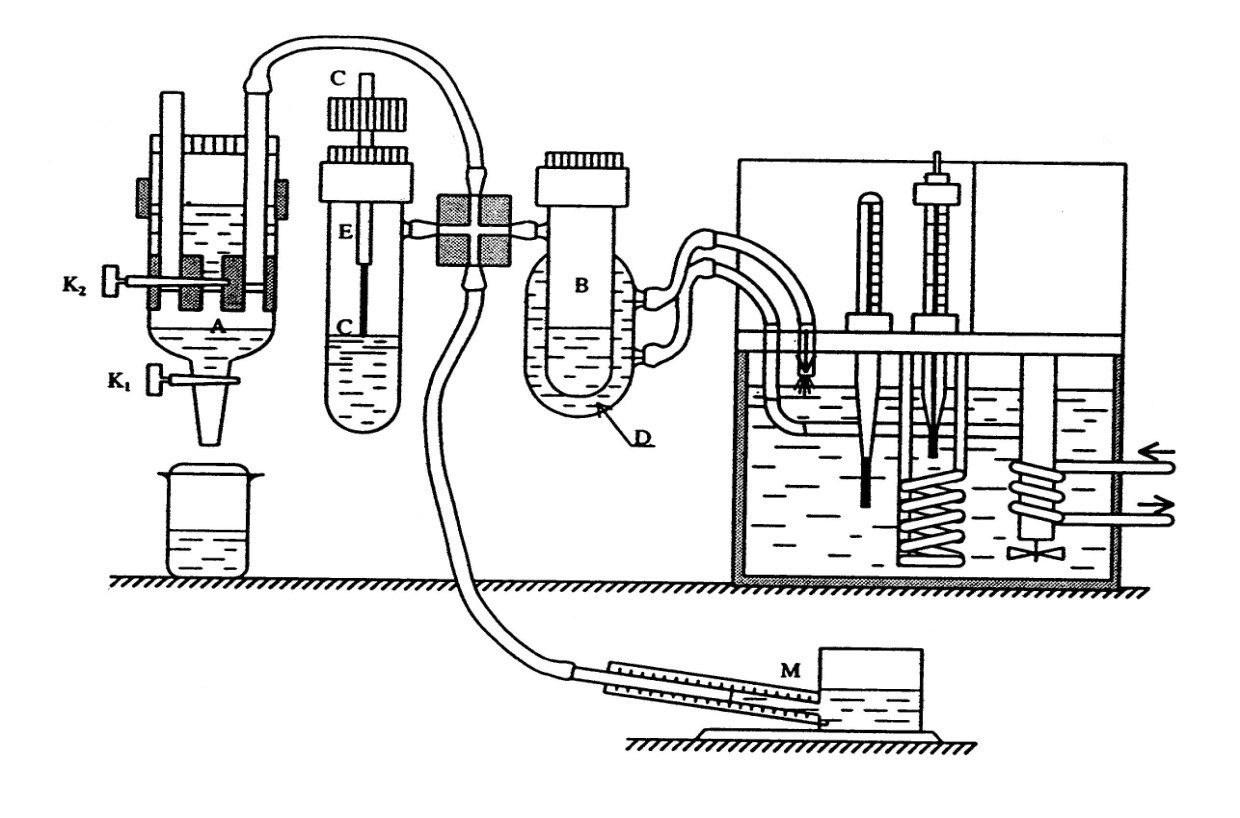
\includegraphics[width=5.9cm]{fac}
			\caption{Рисунок экспериментальной установки}
			\label{img:ust}
		\end{center}
	\end{wrapfigure}
	
	Исследуемая жидкость (дистиллированная вода) наливается в сосуд (колбу) $ B $ (рис. \eqref{img:ust}). Тестовая жидкость  (этиловый спирт) наливается  в сосуд $ E $.  При измерениях  колбы герметично закрываются  пробками. Через одну из двух пробок  проходит полая металлическая игла $ С $. Этой пробкой закрывается сосуд, в котором  проводятся измерения. Верхний конец иглы открыт в атмосферу, а нижний погружен в жидкость. Другой сосуд герметично закрывается второй пробкой. При создании достаточного  разряжения воздуха в колбе с иглой пузырьки воздуха начинают пробулькивать через жидкость. Поверхностное натяжение можно определить по величине разряжения $ \Delta P $ \eqref{key}, необходимого для прохождения пузырьков (при известном радиусе иглы).
	
	Разряжение в системе создается с помощью аспиратора $ A $. Кран $ K_2 $ разделяет две полости аспиратора. Верхняя полость при закрытом кране $ K_2 $ заполняется водой. Затем кран $ K_2 $ открывают и заполняют водой  нижнюю полость  аспиратора.  Разряжение воздуха создается в нижней полости  при открывании крана $ K_1 $, когда  вода вытекает из неё по каплям. В колбах $ В $ и $ С $, соединённых трубками с нижней полостью аспиратора, создается такое же пониженное давление. Разность давлений в полостях с разряженным воздухом и атмосферой измеряется спиртовым микроманометром. 
	
	Для стабилизации температуры исследуемой жидкости через рубашку $ D $ колбы $ В $ непрерывно прогоняется вода из термостата.
	
	Обычно кончик иглы лишь касается поверхности жидкости, чтобы исключить влияние гидростатического давления столба жидкости. Однако при измерении температурной зависимости коэффициента поверхностного натяжения возникает ряд сложностей. Во-первых, большая теплопроводность металлической трубки приводит к тому, что температура на конце трубки заметно ниже, чем в глубине жидкости. Во-вторых, тепловое расширение поднимает уровень жидкости при увеличении температуры.
	
	Обе погрешности можно устранить, погрузив кончик трубки до самого дна. Полное давление, измеренное при этом микроманометром, равно \[ P = \Delta P + \rho g h.\] Заметим, что $ \rho gh $ от температуры практически не зависит, так как подъём уровня жидкости компенсируется уменьшением её плотности (произведение $ \rho g $ определяется массой всей жидкости и поэтому постоянно). Величину  $ \rho g h $ следует измерить двумя способами.
	
	Во-первых, замерить величину $ P_1= \Delta P' $, когда кончик трубки только касается поверхности жидкости. Затем при этой же температуре опустить иглу до дна и замерить $ P_2= \rho gh + \Delta P'' $ ($ \Delta P' $, $ \Delta P'' $ -- давление Лапласа). Из-за  несжимаемости  жидкости можно положить $ \Delta P' = \Delta P'' $ и тогда \[ \rho gh= P_2 - P_1. \]
	
	Во-вторых, при измерениях $ P_1 $ и $ P_2 $ замерить линейкой  глубину погружения иглы $ h $. Это можно сделать, замеряя расстояние между верхним концом иглы и любой неподвижной частью прибора при положении иглы на поверхности и в глубине колбы.
	
	\section{Ход работы}
	\subsection{Измерение диаметра иглы}
	Измерим максимальное давление при пробулькивании пузырьков воздуха через спирт:
	\bgroup
	\def\arraystretch{1.7}%
	\begin{table}[H]
		\begin{center}
			\begin{tabular}{|c|c|c|c|c|c|c|c|c|c|c|c|c|c|c|c|c|}
				\hline
				$P',$ дел. &42&42&42&42&42&42&42&42&43&43&43&43&43&43&43&43\\
				\hline
				$P,$ Па& \multicolumn{8}{c|}{82.4}&\multicolumn{8}{c|}{84.4}\\
				\hline
				$P_{\text{макс}}$& \multicolumn{16}{c|}{83.4}\\
				\hline
				$\sigma_P,$ Па&\multicolumn{16}{c|}{$\sqrt{\left(\sigma_P^\text{сист}\right)^2 + \left(\sigma_P^\text{случ}\right)^2} = \sqrt{2^2 + 0.25^2} \approx 2$}\\
				\hline
			\end{tabular}
		\end{center}
		\caption{Результаты измерений в спирте}
		\label{tab1}
	\end{table}
	\egroup
	
	По формуле \eqref{key} найдем диаметр иглы:
	\begin{equation*}
		d = \frac{4\sigma_{\text{с}}}{P_\text{макс}} = (1.09\pm 0.03)\text{ мм}.
	\end{equation*}

	Результат полученный под микроскопом: $D = (1,00\pm0.05)$ мм, это означает, что диаметр найденный экспериментально достаточно точен.
	
	\subsection{Измерение температурной зависимости коэффициента поверхностного натяжения}
	
	Снимать будем двумя способами: при касании поверхности воды и при полном погружении иглы.
	
	Глубина погружения измеренная линейкой: $\Delta h = (1.30\pm0.07)$ см. Глубина погружения по разнице давлений из первого опыта: $\Delta P = (174-111)*0.2*9.81 = 63\pm0.7$, $\Delta h = \dfrac{\Delta P}{\rho g} = (1.26\pm0.02)$.
	
	Пара таблиц данных (включать все, на мой взгляд, не целесообразно):
	\begin{table}[H]
		\centering
		\begin{minipage}{.49\linewidth}
			\centering
			\bgroup
			\def\arraystretch{1.2}
				\begin{tabular}{|c|c|c|c|}
					\hline
					\multicolumn{4}{|c|}{$T = 23 ^\circ$С}\\
					\hline
					\multicolumn{2}{|c|}{Вверху}&\multicolumn{2}{c|}{Внизу}\\
					\hline
					$P',$ Па& $P,$ Па &$P',$ Па& $P,$ Па\\
					\hline
					111.0&217.7&174.0&341.4\\
					\hline
					111.0&217.7&174.0&341.4\\
					\hline
					111.0&217.7&174.0&341.4\\
					\hline
					111.0&217.7&174.0&341.4\\
					\hline
					111.0&217.7&174.0&341.4\\
					\hline
					111.0&217.7&174.0&341.4\\
					\hline
				\end{tabular}
			\egroup
		\end{minipage}
		\begin{minipage}{.49\linewidth}
			\centering
			\bgroup
			\def\arraystretch{1.2}%
				\begin{tabular}{|c|c|c|c|}
					\hline
					\multicolumn{4}{|c|}{$T = 65.3 ^\circ$С}\\
					\hline
					\multicolumn{2}{|c|}{Вверху}&\multicolumn{2}{c|}{Внизу}\\
					\hline
					$P',$ Па& $P,$ Па &$P',$ Па& $P,$ Па\\
					\hline
					98.0& 192.3&165.0&323.7\\
					\hline
					98.0& 192.3&165.0&323.7\\
					\hline
					98.0& 192.3&165.0&323.7\\
					
					\hline
					99.0& 194.2&165.0&323.7\\\hline
					99.0& 194.2&165.0&323.7\\
					\hline
					99.0& 194.2&165.0&323.7\\
					\hline
				\end{tabular}
			\egroup
		\end{minipage}
		\caption{Результаты измерений для воды}
		\label{water}
	\end{table}

	Рассчитывать коэффициент поверхностного натяжения будем по формуле:
	\begin{equation*}
		\sigma = \frac{\Delta P d}{4}.
	\end{equation*}
	Для измерений при опущенной игле учитываем глубину погружения, то есть $\Delta P = P - \rho g h.$
	
	Получаем таблицы:
		\begin{table}[H]
			\bgroup
			\def\arraystretch{1.2}%
			\begin{minipage}{0.49\linewidth}
			
			\centering
			\begin{tabular}{|c|c|c|}
				\hline
				\multicolumn{3}{|c|}{Внизу}\\
				\hline
				$P',$ Па&$\sigma,\: \frac{\text{мН}}{\text{м}}$& $T,\: ^\circ$С  \\
				\hline
				173 & 54.0$\pm$0.5 & 25 \\ \hline
				172 & 53.5$\pm$0.5 & 30.5 \\ \hline
				171 & 53.0$\pm$0.5 & 35.5 \\ \hline
				170 & 52.5$\pm$0.5 & 40.5 \\ \hline
				169 & 52.0$\pm$0.5 & 45.5 \\ \hline
				168 & 51.5$\pm$0.5 & 50.2 \\ \hline
				167 & 51.0$\pm$0.5 & 55.2 \\ \hline
				166 & 50.5$\pm$0.5 & 60.3 \\ \hline
				165 & 50.0$\pm$0.5 & 65.3 \\ \hline
			\end{tabular}
			\end{minipage}
			\begin{minipage}{0.49\linewidth}
				\centering
					\begin{tabular}{|c|c|c|}
						\hline
						\multicolumn{3}{|c|}{Вверху}\\
						\hline
						
						$P',$ Па&$\sigma,\: \frac{\text{мН}}{\text{м}}$& $T,\: ^\circ$С  \\
						\hline
						111 & 54.5 & 23 \\ \hline
						107 & 52.5 & 35.5 \\ \hline
						105.75 & 51.9 & 40.6 \\ \hline
						104 & 51.1 & 45.5 \\ \hline
						100 & 49.1 & 50.2 \\ \hline
						100 & 49.1 & 55.2 \\ \hline
						100 & 49.1 & 60.3 \\ \hline
						98.6 & 48.4 & 65.3 \\ \hline
					\end{tabular}

			\end{minipage}
			\egroup
		\end{table}
	Строим по ним графики зависимости $\sigma(T)$:
	\begin{figure}[H]
		\centering
		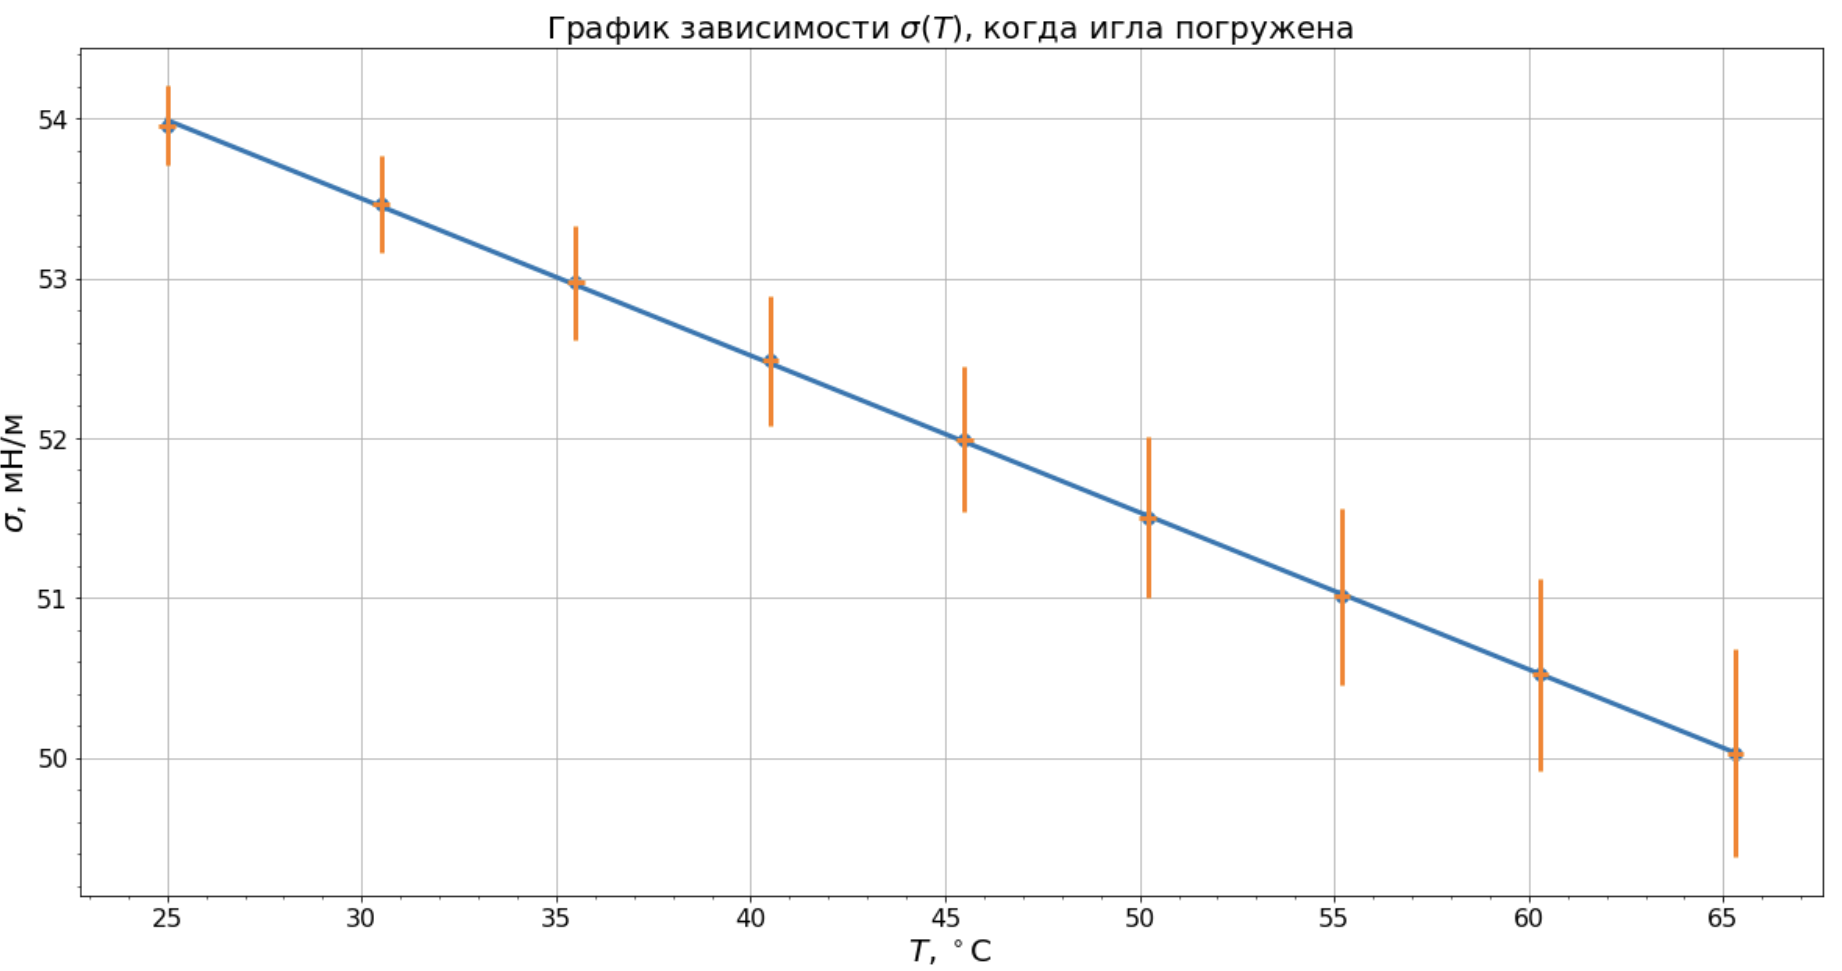
\includegraphics[scale = 0.55]{down}
		\caption{График зависимости $\sigma(T)$, для погруженной иглы}
		\label{graph1}
	\end{figure}
	\begin{figure}[H]
		\centering
		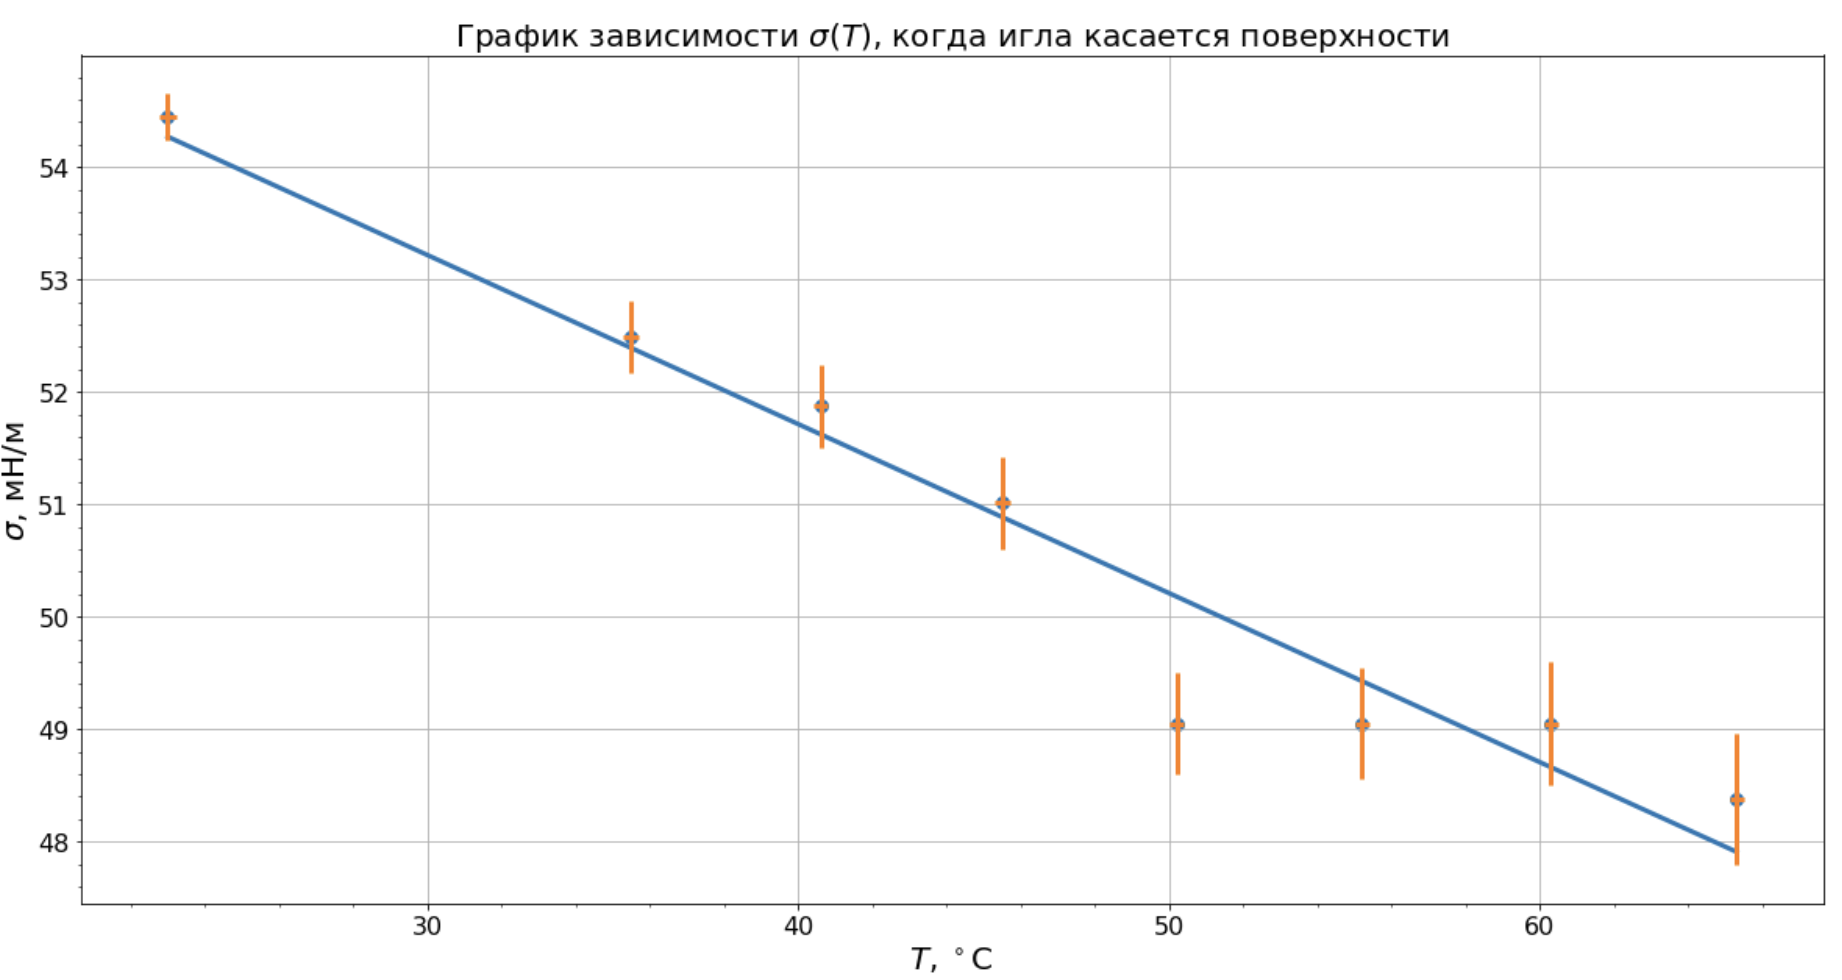
\includegraphics[scale = 0.55]{up}
		\caption{График зависимости $\sigma(T)$, для поднятой иглы}
		\label{graph2}
	\end{figure}
	
	Температурные коэффициенты $\left(\dfrac{d\sigma}{dT}\right)$:
	\begin{enumerate}
		\item Погруженная игла: $k = (-9.8\pm 0.5)\cdot 10^{-2}$ $\dfrac{\text{мН}}{\text{м}\cdot \text{К}}$, $\varepsilon \approx 5.1\%$.
		\item Поднятая игла: $k = (-15.0\pm 1.5)\cdot 10^{-2}$ $\dfrac{\text{мН}}{\text{м}\cdot \text{К}}$, $\varepsilon \approx 10.2\%$.
	\end{enumerate}

	\subsection{Графики других величин}
	
	Окончательно, с помощью полученных данных построим графики теплоты образования единицы поверхности жидкости: $q = - T\cdot\dfrac{d\sigma}{dT}$ и поверхностной энергии $U$ единицы площади $F$: $\dfrac{U}{F} = \left(\sigma - T\cdot\dfrac{d\sigma}{dT}\right)$.
	
	Графики построены используя данные погруженной иглы:
	\begin{table}[H]
		\centering
		\begin{minipage}{.49\linewidth}
			\centering
			\begin{figure}[H]
				\centering
				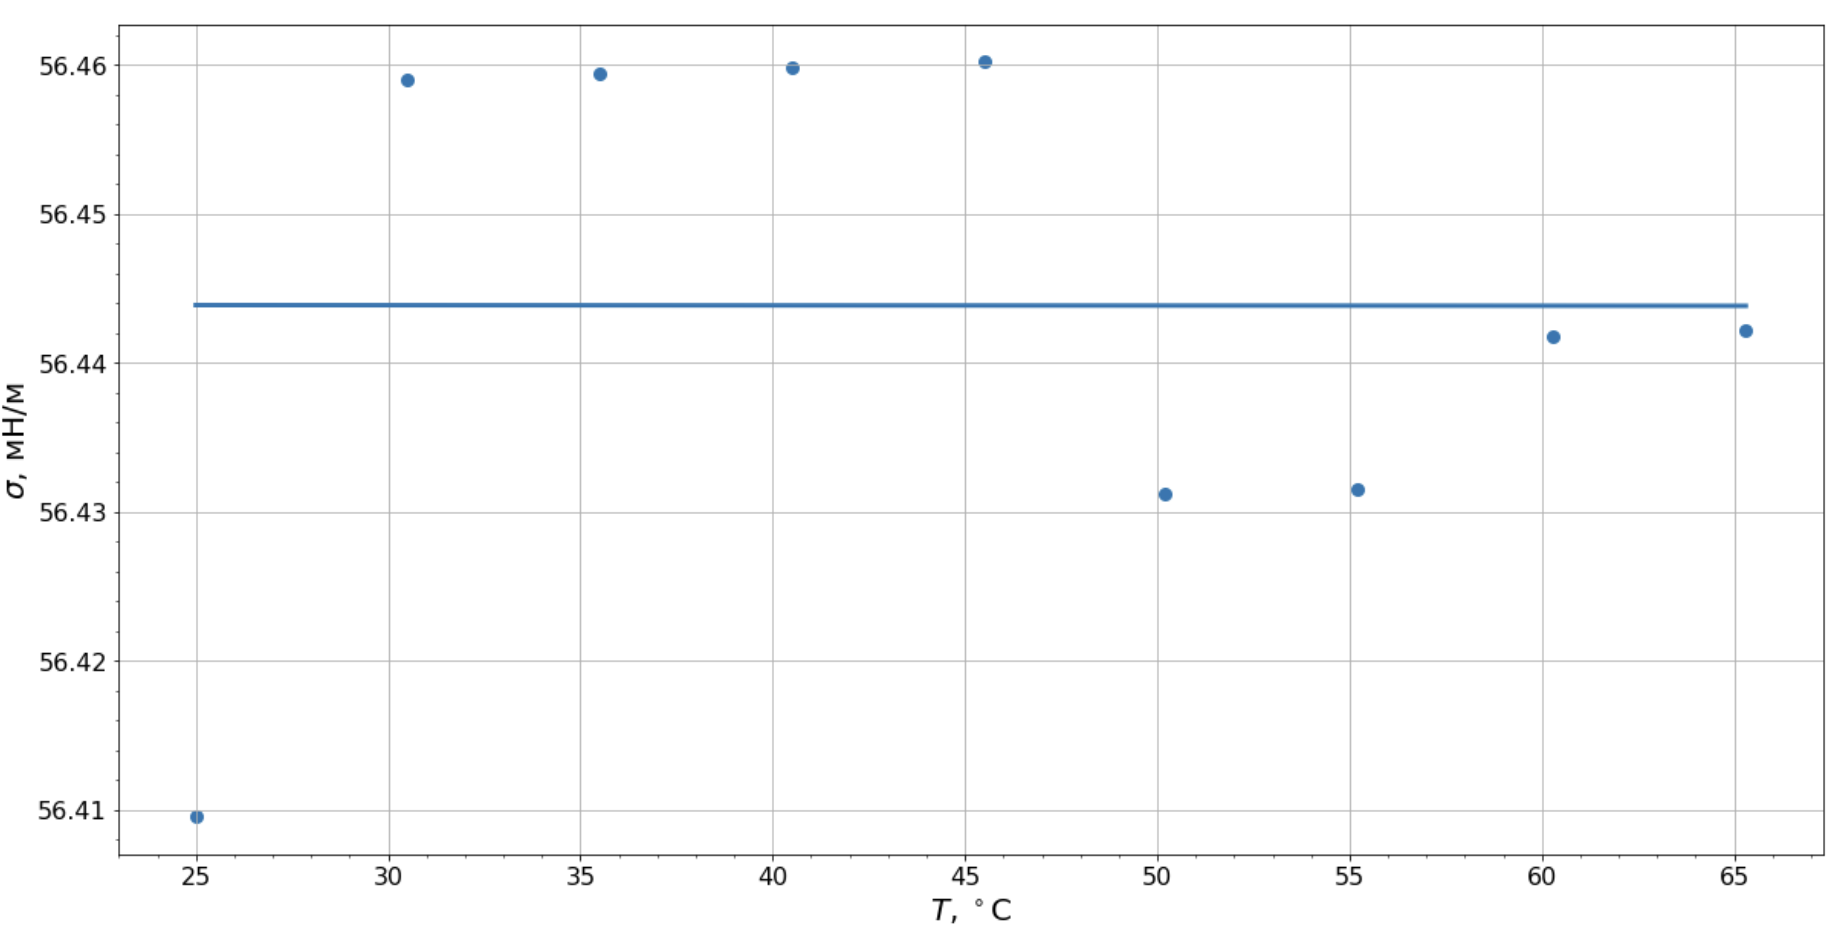
\includegraphics[scale = 0.25]{u}
				\caption{График $\dfrac{U}{F}$}
				\label{graph4}
			\end{figure}
		\end{minipage}
		\begin{minipage}{.49\linewidth}
			\centering
			\begin{figure}[H]
				\centering
				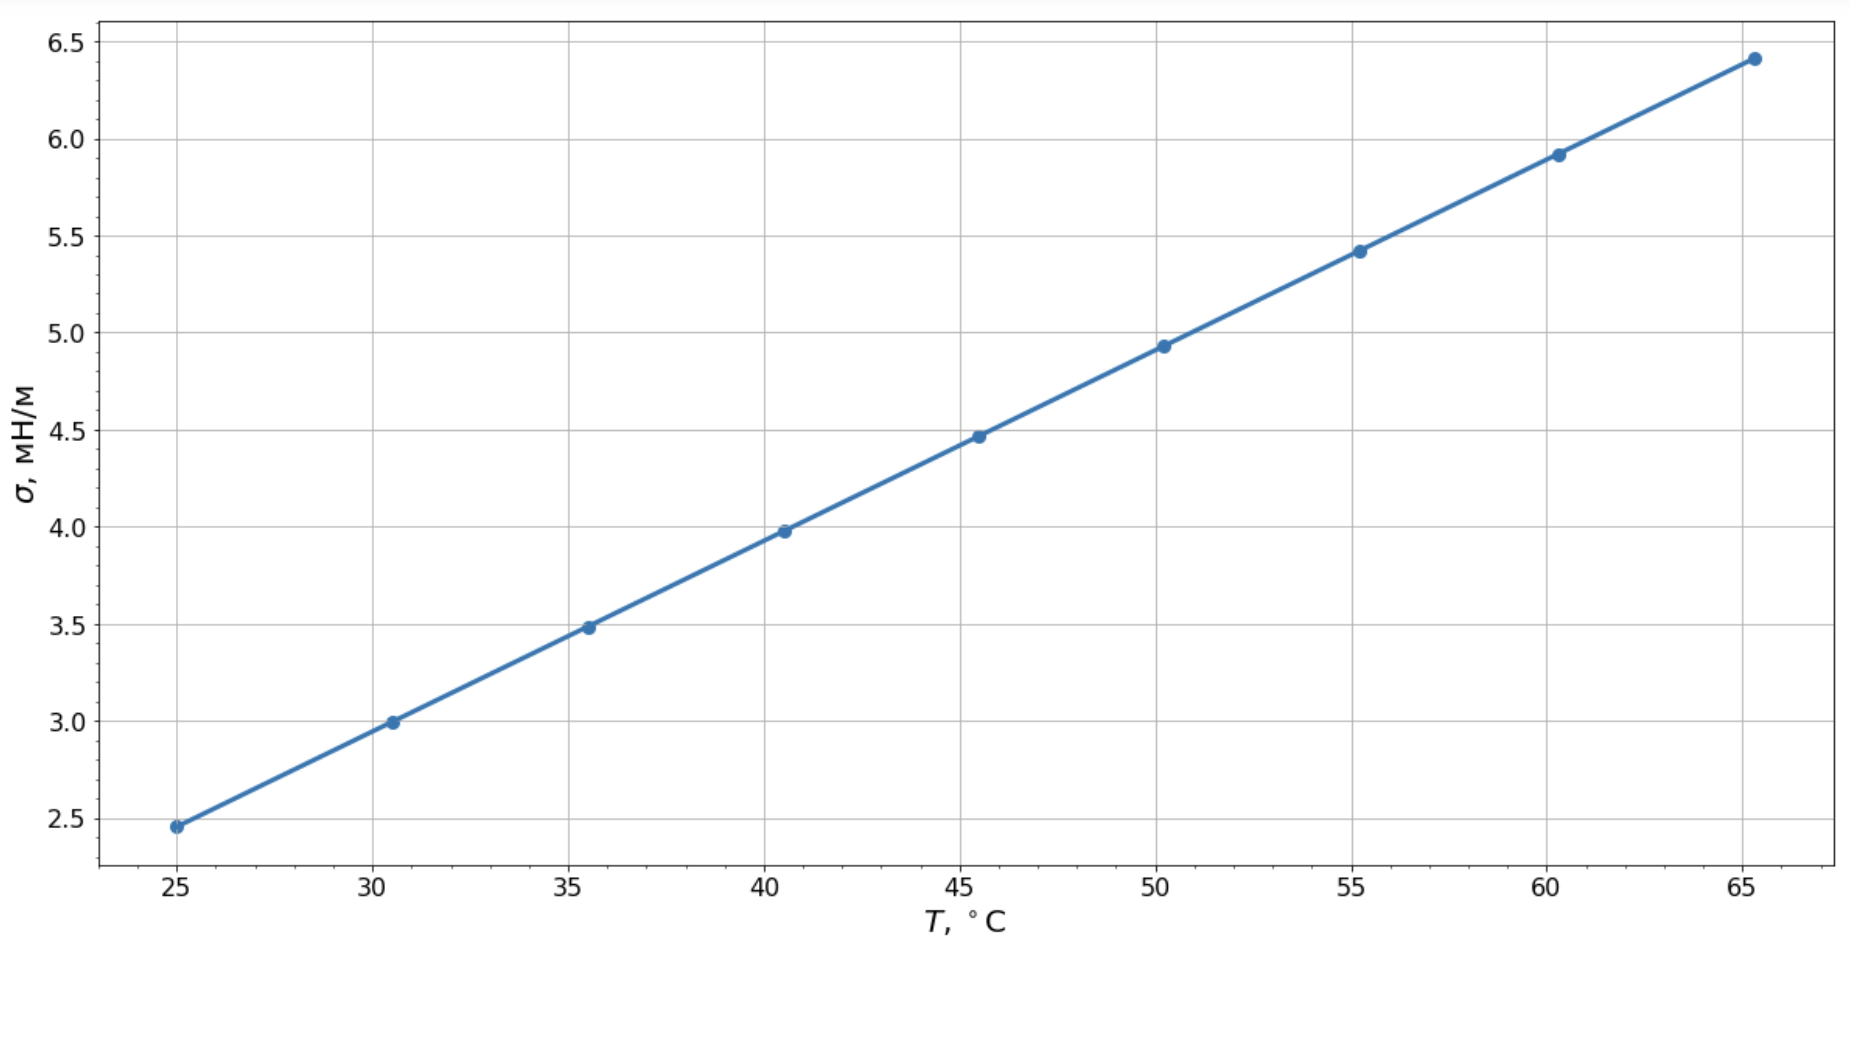
\includegraphics[scale = 0.25]{q}
				\caption{График $q$}
				\label{graph5}
			\end{figure}
		\end{minipage}
	\end{table}

	\section{Вывод}
	В ходе работы:
	\begin{enumerate}
		\item Был экспериментально измерен диаметр иглы при помощи коэффициента поверхностного натяжения спирта. Полученный результат $d = (1.09\pm 0.03)\text{ мм}$ с достаточной точность совпадает с диаметром измеренным с помощью микроскопа.
		\item Было измерено давление, создаваемое столбом жидкости при опускании иглы на $\Delta h = (1.3\pm 0.1)$ см.
		\item Получены коэффициенты поверхностного натяжения воды при различных ее температурах, например $\sigma = (54.0\pm 0.5)\:\frac{\text{мН}}{\text{м}}$ при температуре 25 $^\circ$С.
		\item Так же было проведено сравнение воздействия различного положения иглы на результаты. Как мы можем увидеть, намного лучше эксперимент получается, при погруженной нити, так как, я думаю, что она хорошо прогревается вместе с водой, чего не происходит с иглой при касании границы воды.
	\end{enumerate}
	
	
	
	
	
	
	
\end{document}